\documentclass[8pt]{beamer}
\usepackage[slovene]{babel}
\usepackage[utf8]{inputenc}
\usepackage[T1]{fontenc}
\usepackage{lmodern}
\usepackage{mathptmx}
\usepackage{helvet}
\usepackage{courier}
\usepackage{hyperref}
\usepackage{tikz}
\usepackage{enumerate}
\setbeamertemplate{caption}[numbered]

\usetheme{CambridgeUS}

\setbeamercolor*{item}{fg=red}
\setbeamercolor*{label}{fg=red}

\begin{document}


\title[Reševanje TSP s k-opt in LK algoritmom]{Reševanje problema trgovskega potnika s k-optimalnim in
Lin-Kernighanovim algoritmom}
\author[Žan Jernejčič in Ines Šilc]{Žan Jernejčič in Ines Šilc}
\institute [FMF]{Fakulteta za matematiko in fiziko}

\begin{frame}
	\titlepage
\end {frame}

%\begin{frame}
%\begin{minipage}{0.3\textwidth}
%\begin{tikzpicture}
%  [scale=.3,auto=left,every node/.style={circle, draw = black!60}]
%  \node (n0) at (1,8) {0};
%  \node (n1) at (5,10)  {1};
%  \node (n2) at (9,8)  {2};
%  \node (n5) at (1,4) {5};
%  \node (n4) at (5,2)  {4};
%  \node (n3) at (9,4)  {3};
%
%  \foreach \from/\to in {n0/n1,n1/n2,n2/n3,n3/n4,n4/n5,n5/n0}
%    \draw (\from) -- (\to);
%\end{tikzpicture}
%\end{minipage}
%\hspace{0.5cm}
%\begin{minipage}{0.3\textwidth}
%\begin{tikzpicture}
%  [scale=.3,auto=left,every node/.style={circle, draw = black!60}]
%  \node (n0) at (1,8) {0};
%  \node (n1) at (5,10)  {1};
%  \node (n2) at (9,8)  {2};
%  \node (n5) at (1,4) {5};
%  \node (n4) at (5,2)  {4};
%  \node (n3) at (9,4)  {3};
%
%  \foreach \from/\to in {n0/n2,n1/n2,n1/n3,n3/n4,n4/n5,n5/n0}
%    \draw (\from) -- (\to);
%\end{tikzpicture}
%\end{minipage}
%\hspace{0.5cm}
%\begin{minipage}{0.3\textwidth}
%\begin{tikzpicture}
%  [scale=.3,auto=left,every node/.style={circle, draw = black!60}]
%  \node (n0) at (1,8) {0};
%  \node (n1) at (5,10)  {1};
%  \node (n2) at (9,8)  {2};
%  \node (n5) at (1,4) {5};
%  \node (n4) at (5,2)  {4};
%  \node (n3) at (9,4)  {3};
%
%  \foreach \from/\to in {n0/n2,n1/n2,n1/n3,n3/n5,n4/n5,n4/n0}
%    \draw (\from) -- (\to);
%\end{tikzpicture}
%\end{minipage}\\\vspace{0.5cm}
%\end{frame}

\begin{frame}
\begin{equation}
\label{matrika}
\begin{bmatrix} 
0&2&3&4&1000\\
2&0&8&9&10\\
3&8&0&14&15\\
4&9&14&0&20\\
1000&10&15&20&0\\
\end{bmatrix}
\end{equation}
\end{frame}

\begin{frame}
  \begin{figure}
  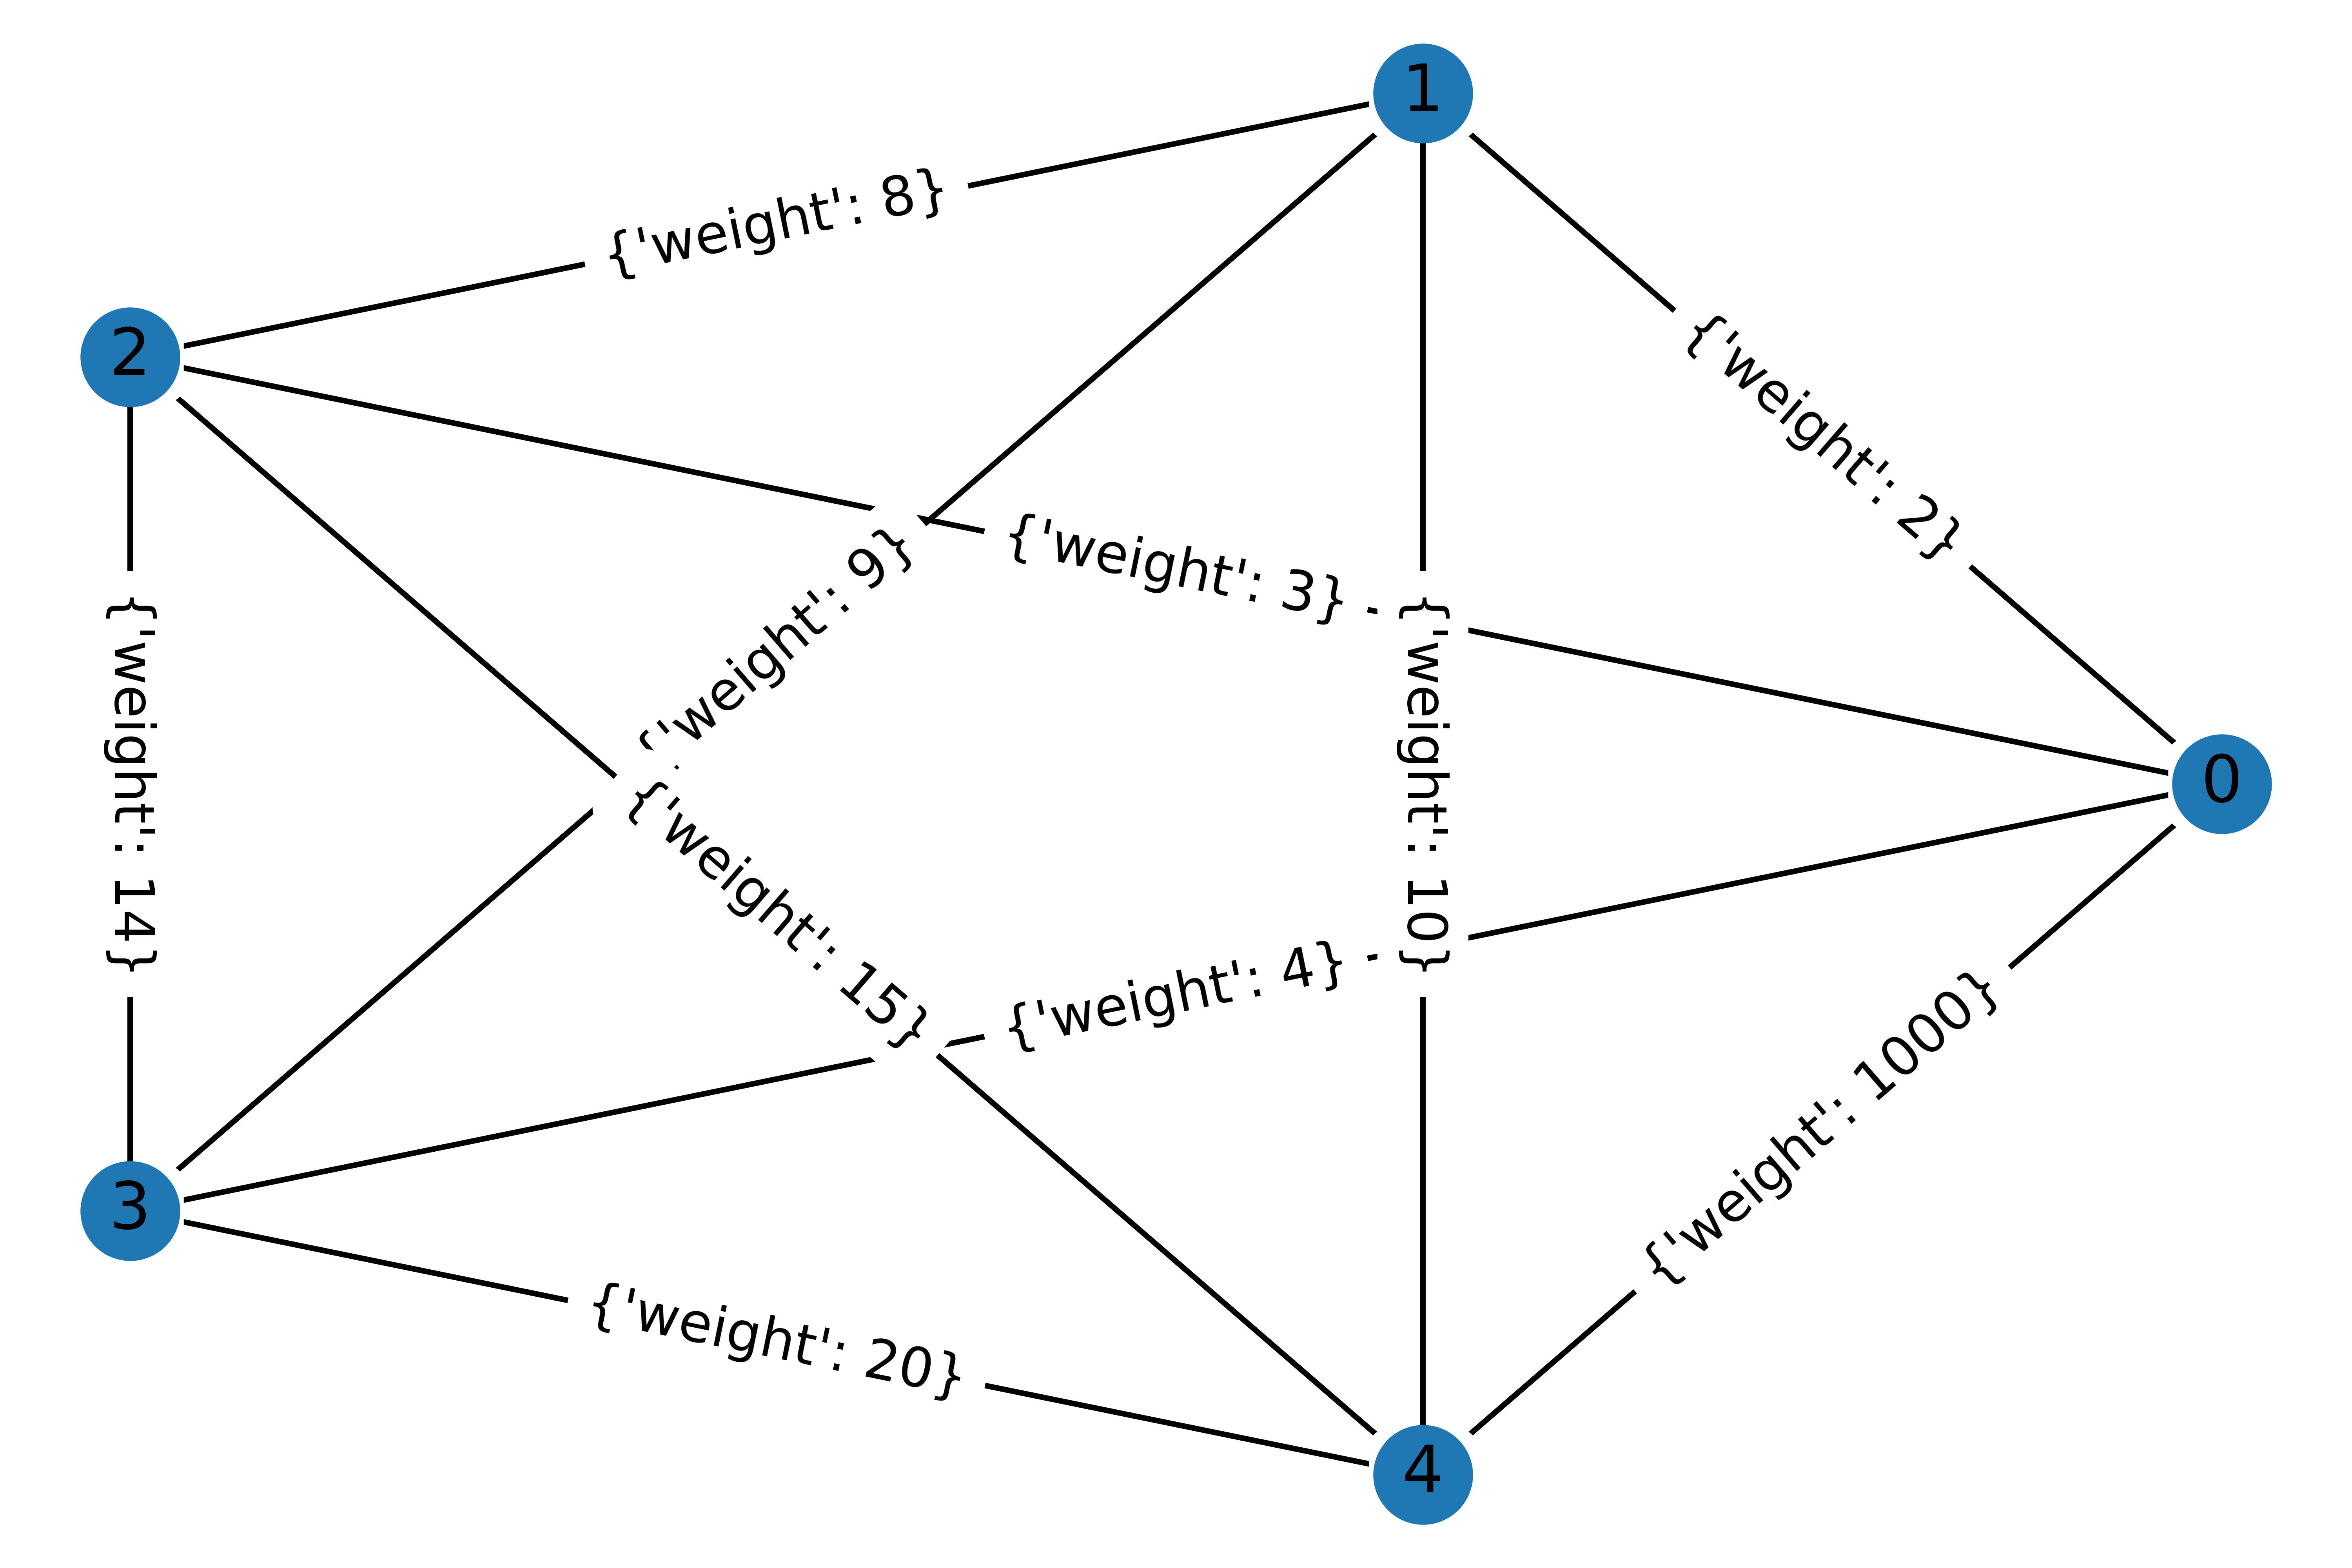
\includegraphics[width=10cm]{primeri/primer1.png}
 	\caption{Poln graf na 5 vozliščih}
	\label{Slika 1}
	\end{figure}
\end{frame}

\begin{frame}
\begin{figure}
  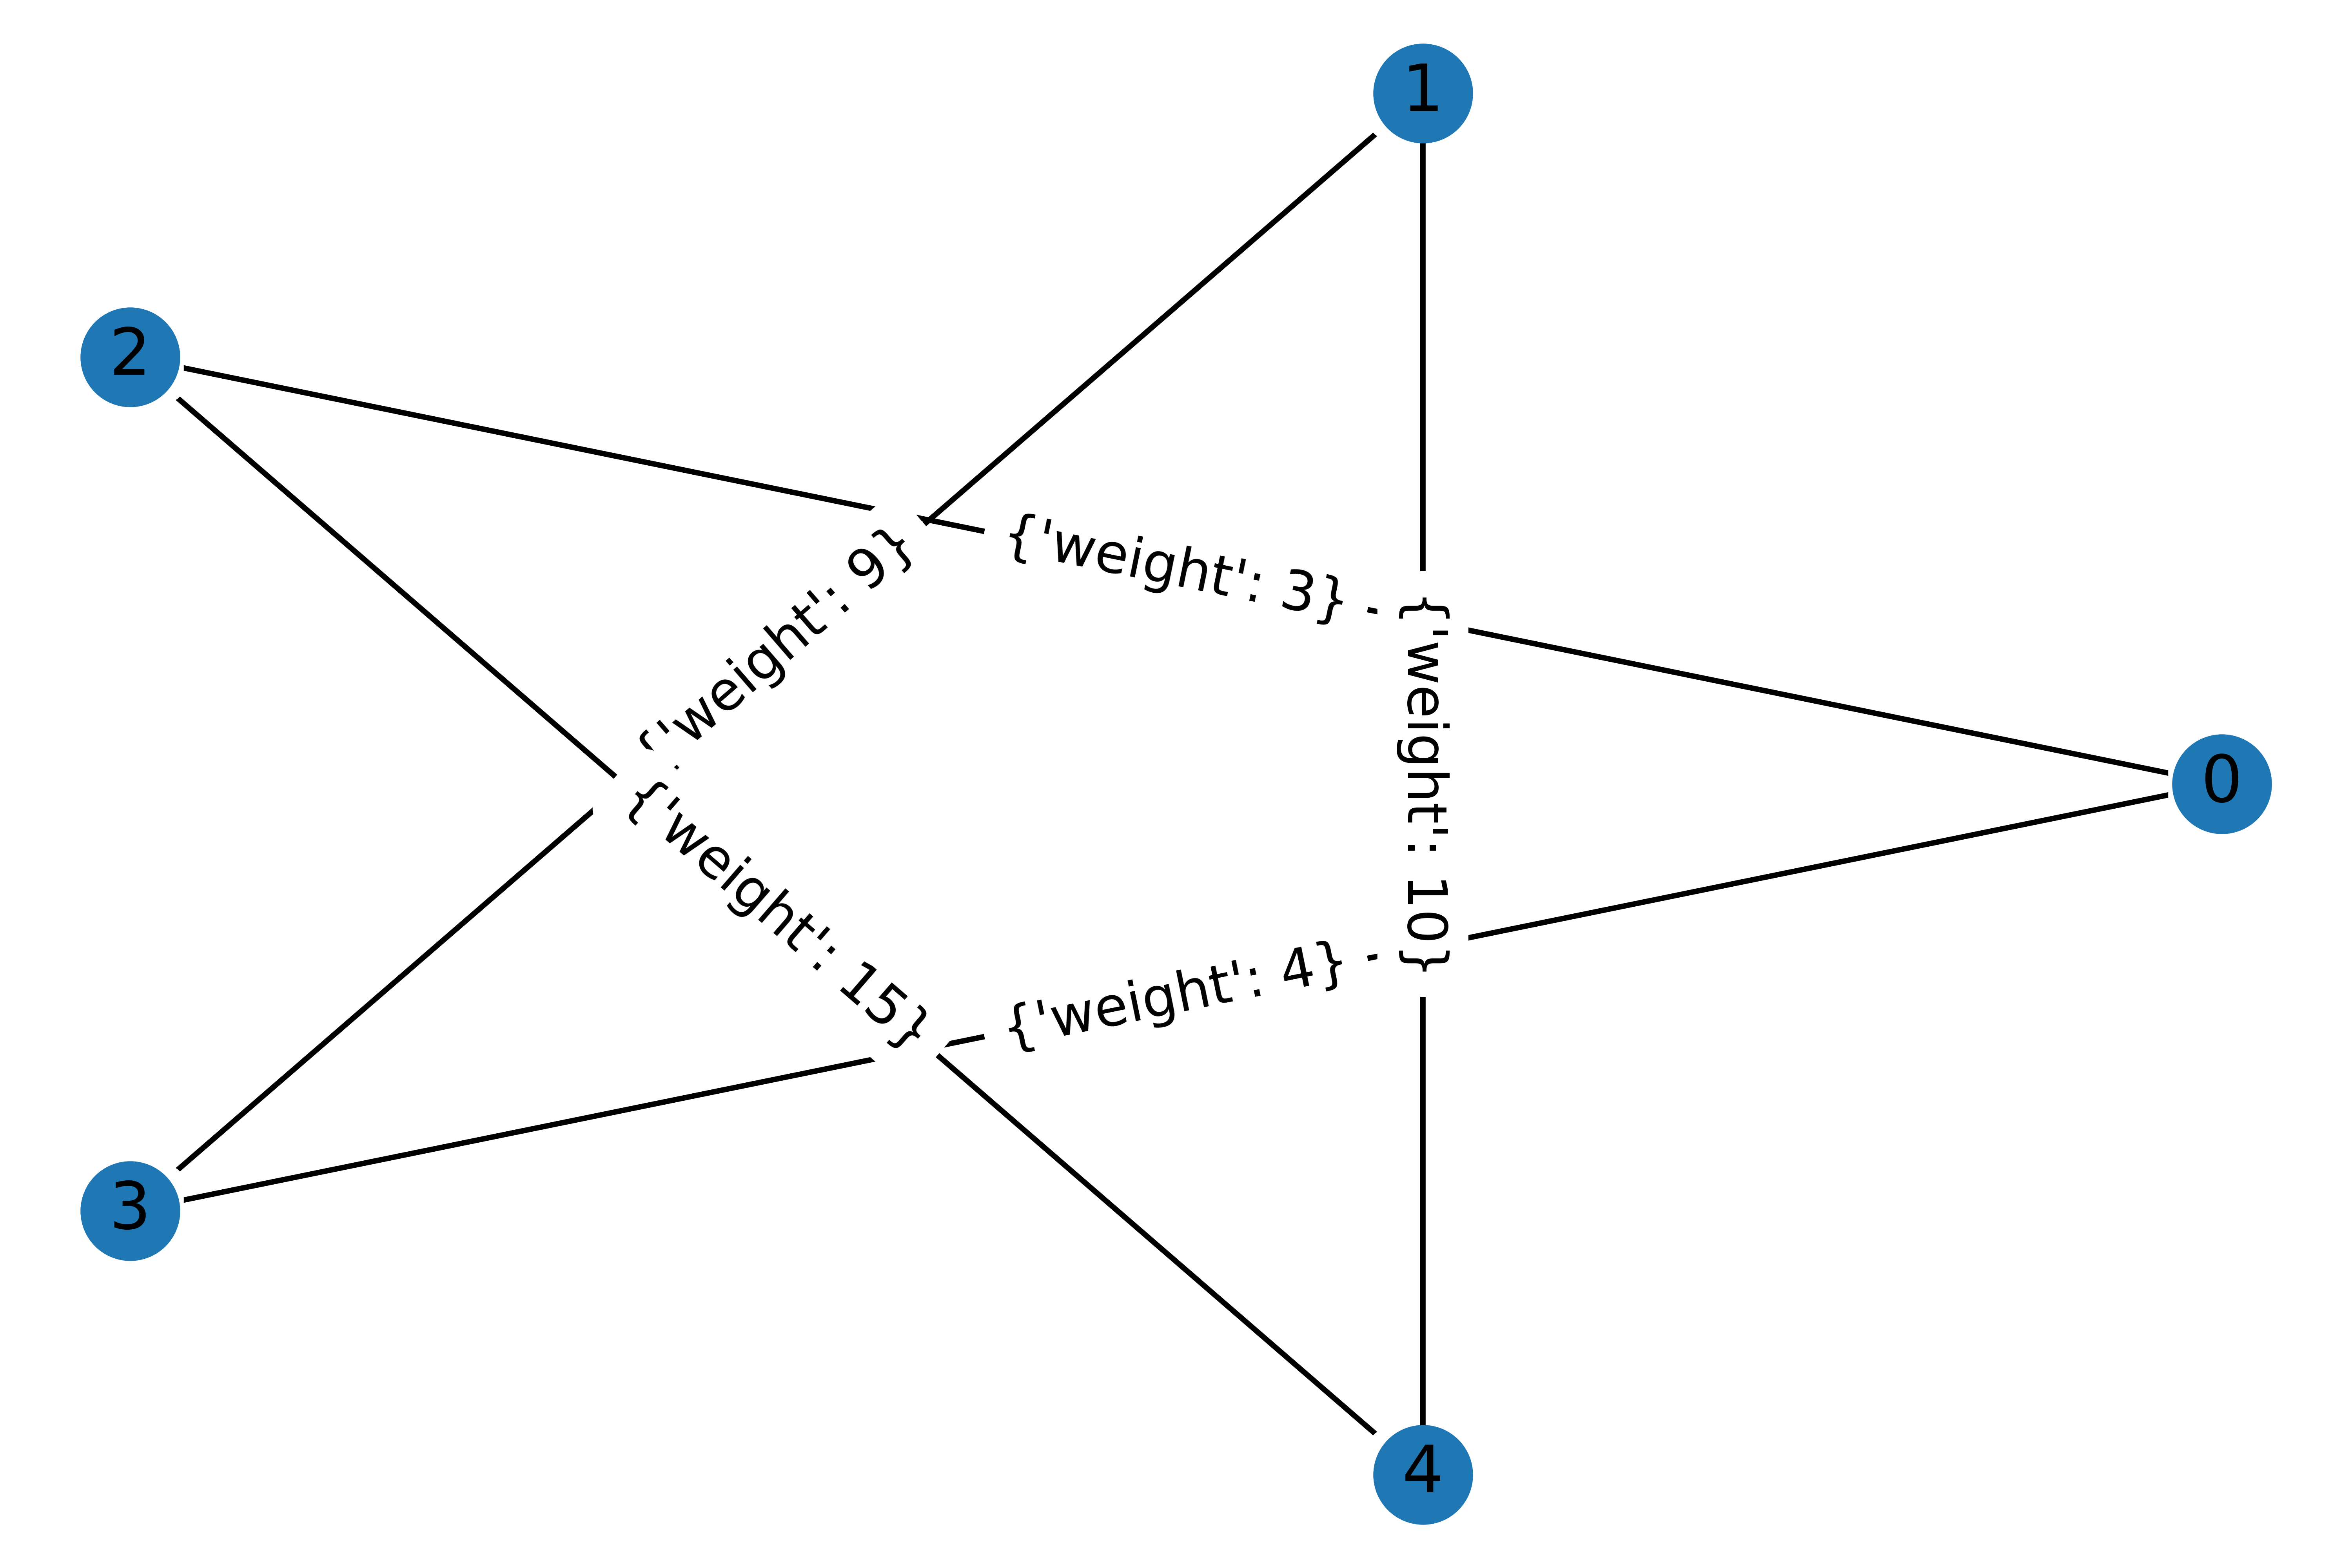
\includegraphics[width=10cm]{primeri/primer1_2opt.png}
\caption{2-opt}
\label{Slika 2}
\end{figure}
\end{frame}

\begin{frame}
  \begin{figure}
  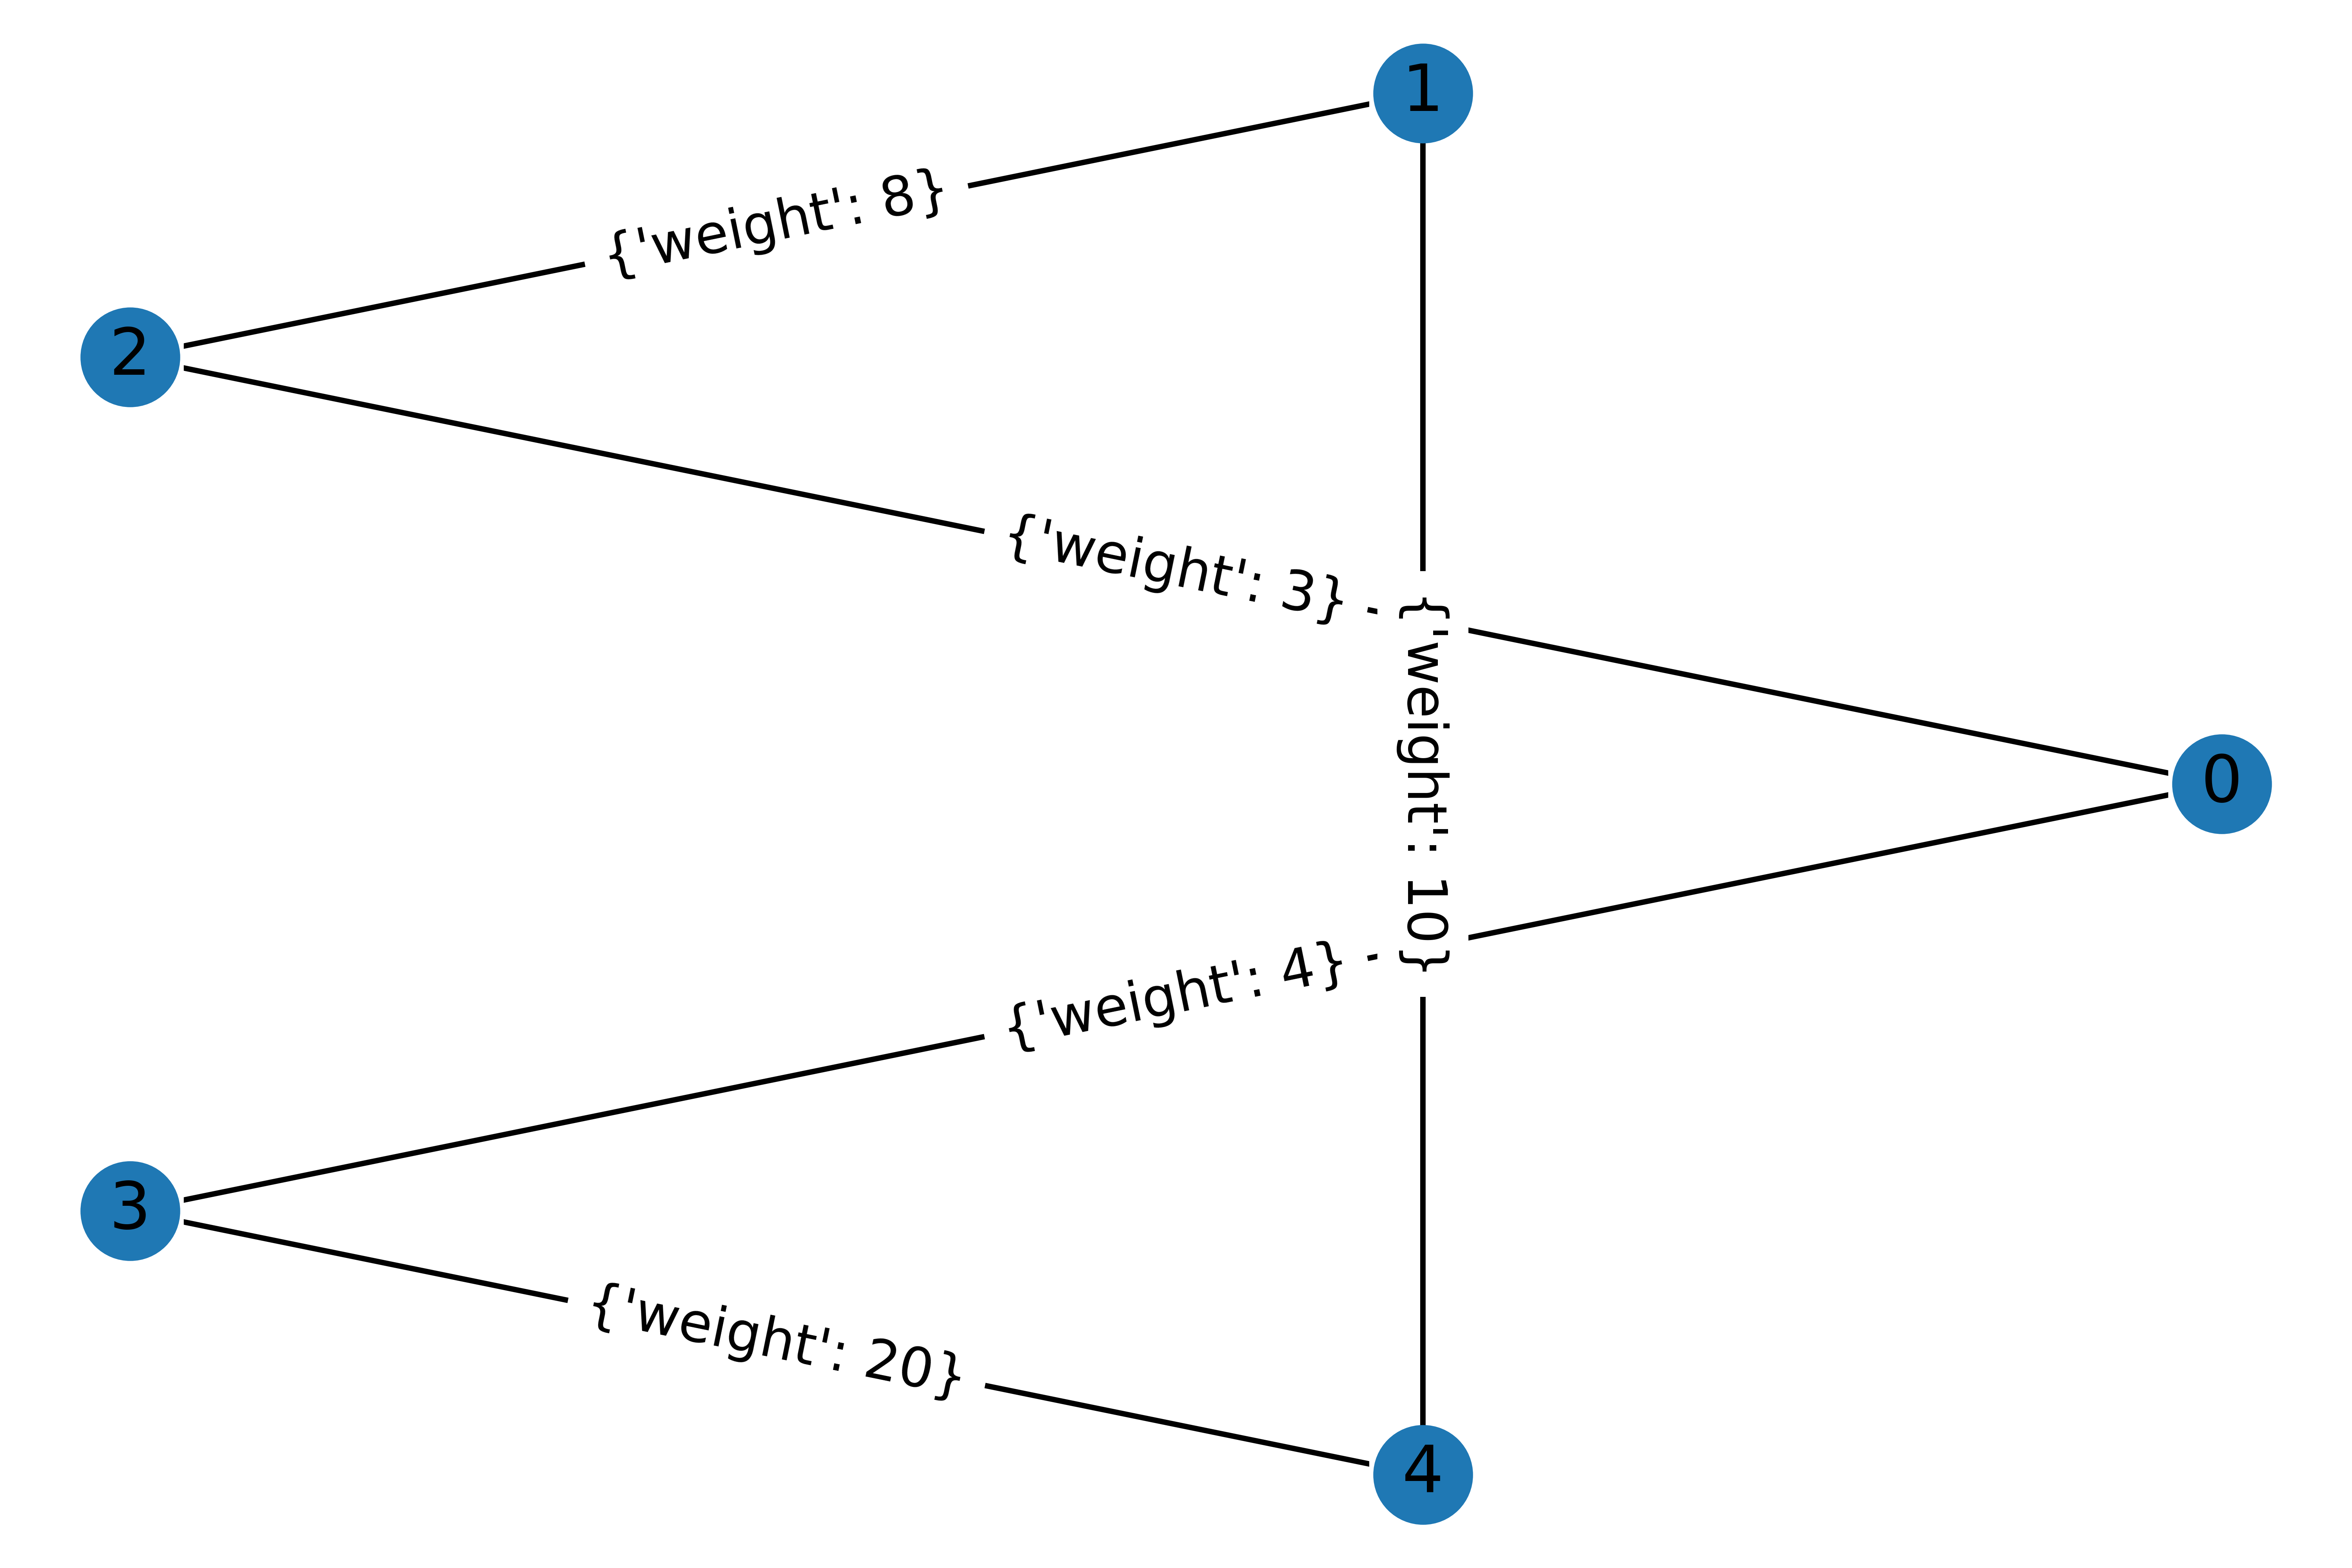
\includegraphics[width=10cm]{primeri/primer1_3opt.png}
 	\caption{3-opt}
	\label{Slika 3}
	\end{figure}
\end{frame}

\begin{frame}
\begin{figure}
  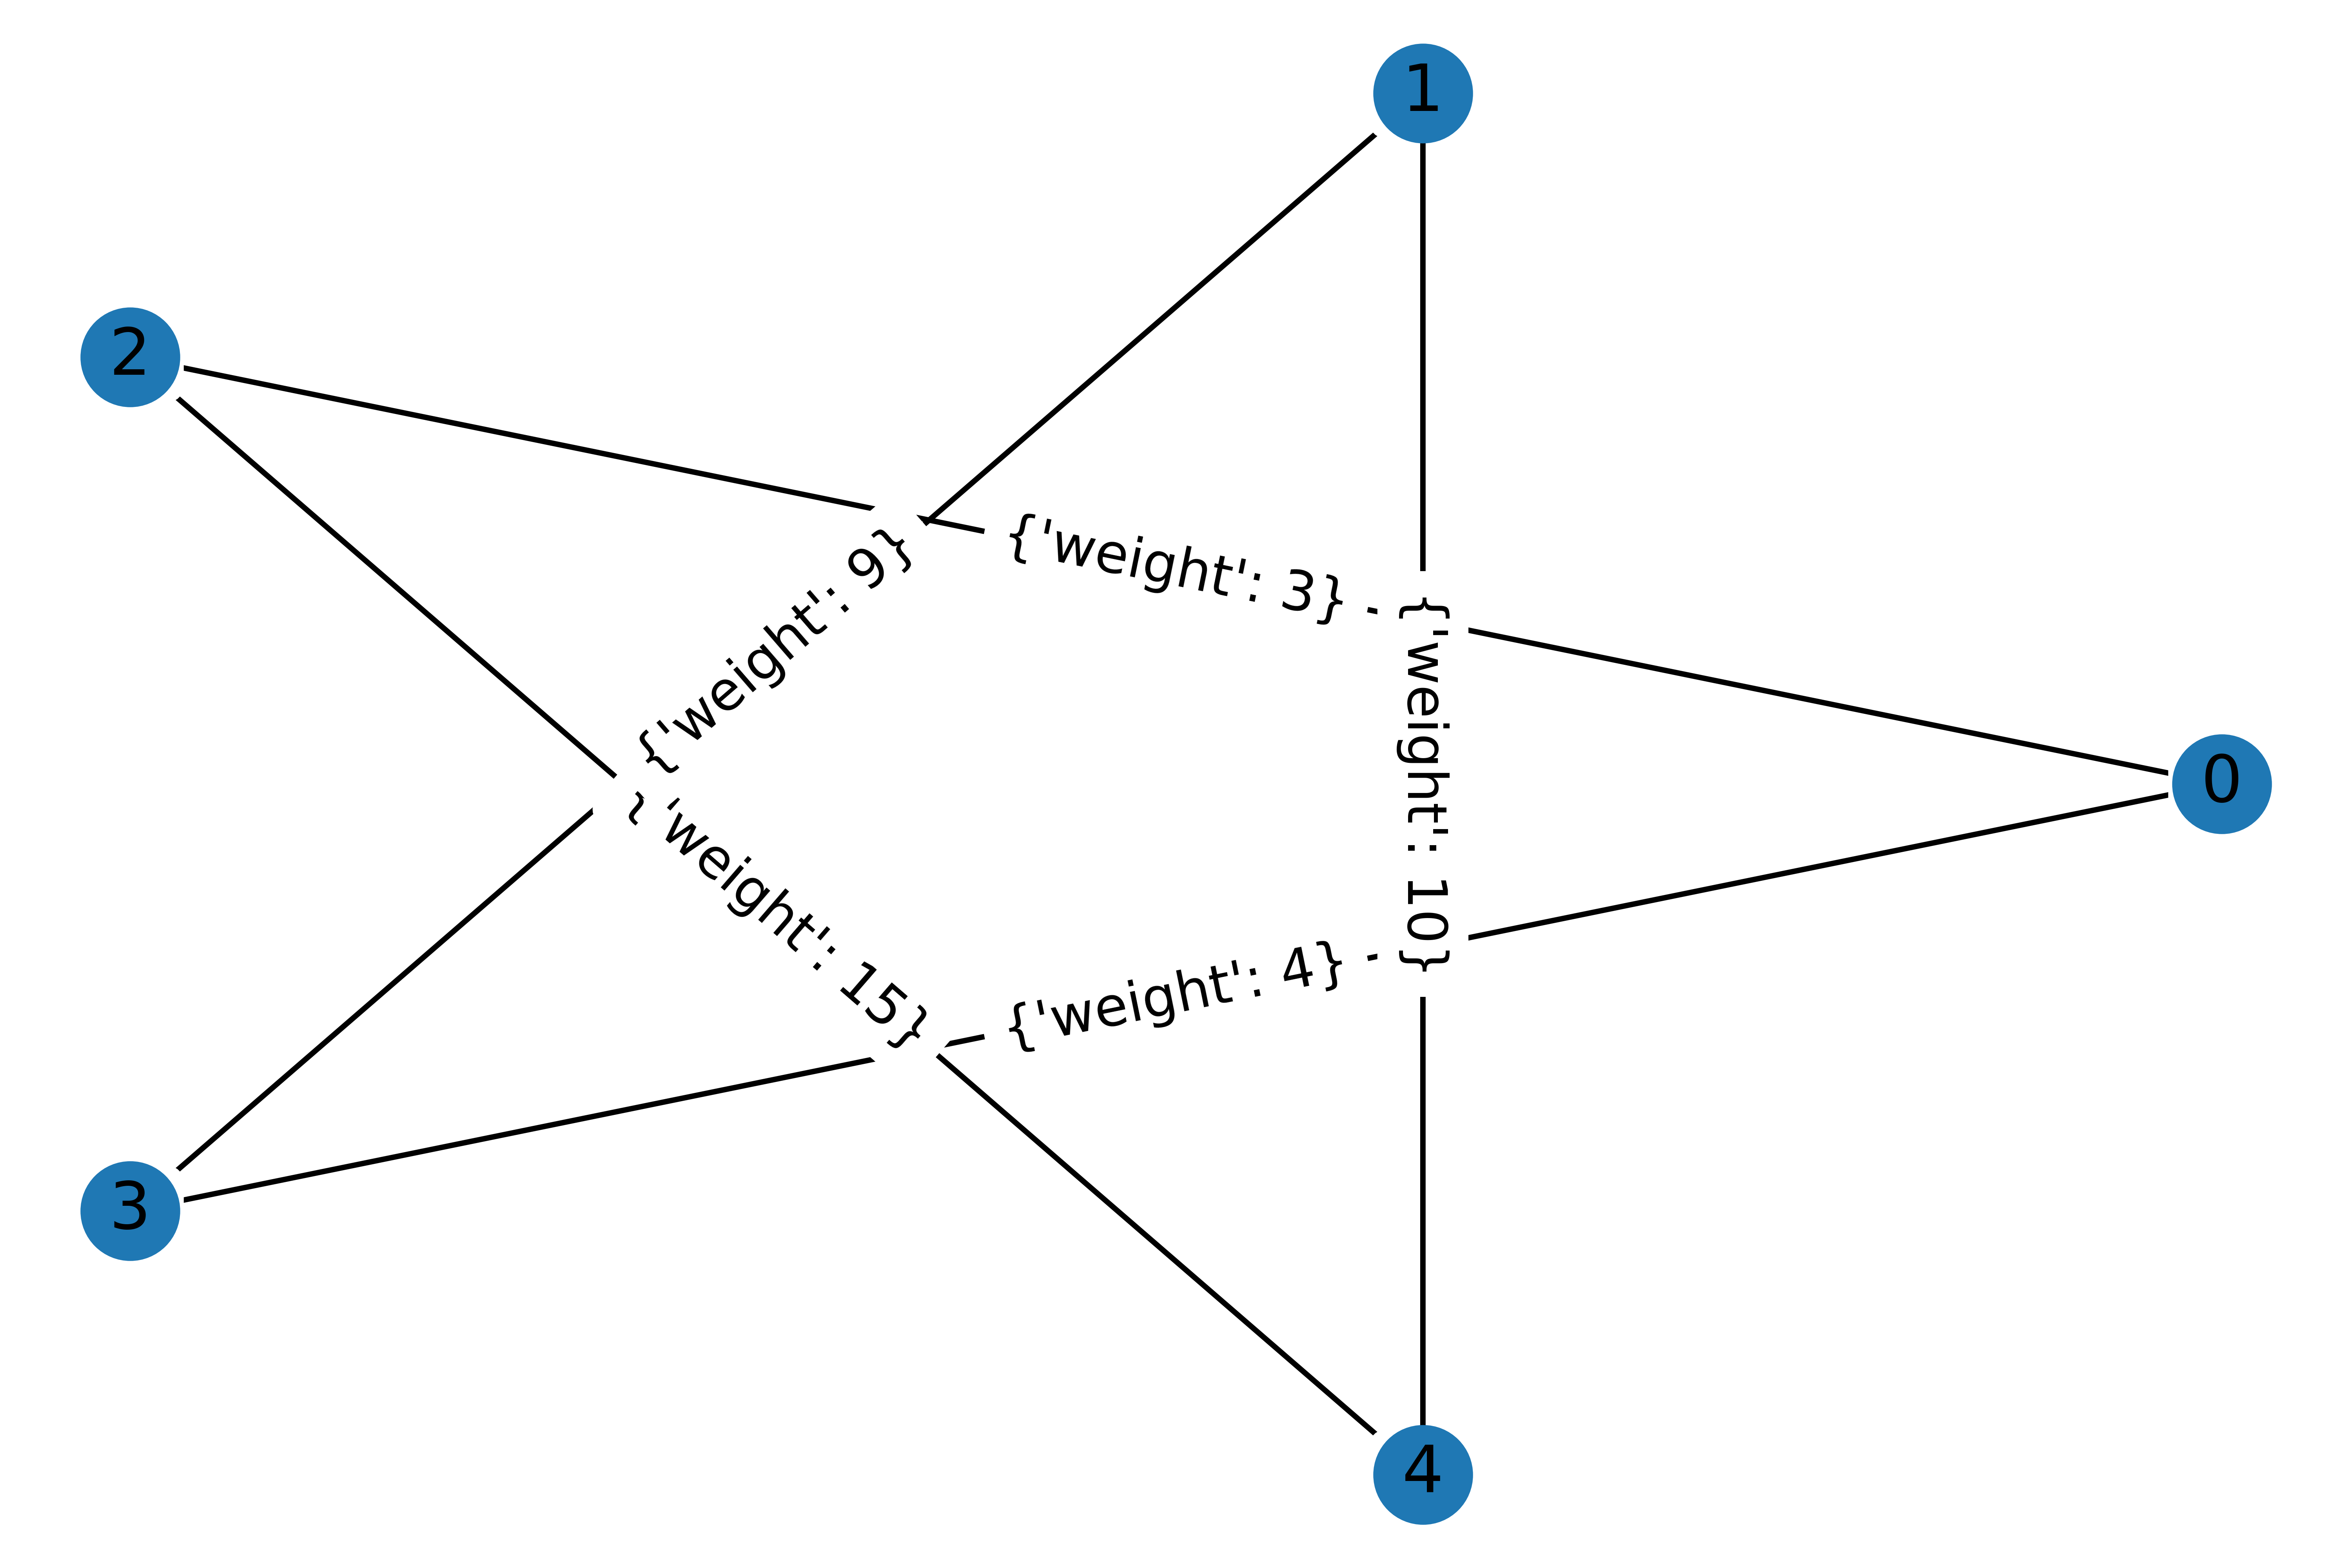
\includegraphics[width=10cm]{primeri/primer1_lk.png}
\caption{LK}
\label{Slika 4}
\end{figure}
\end{frame}

\begin{frame}
  \begin{figure}
  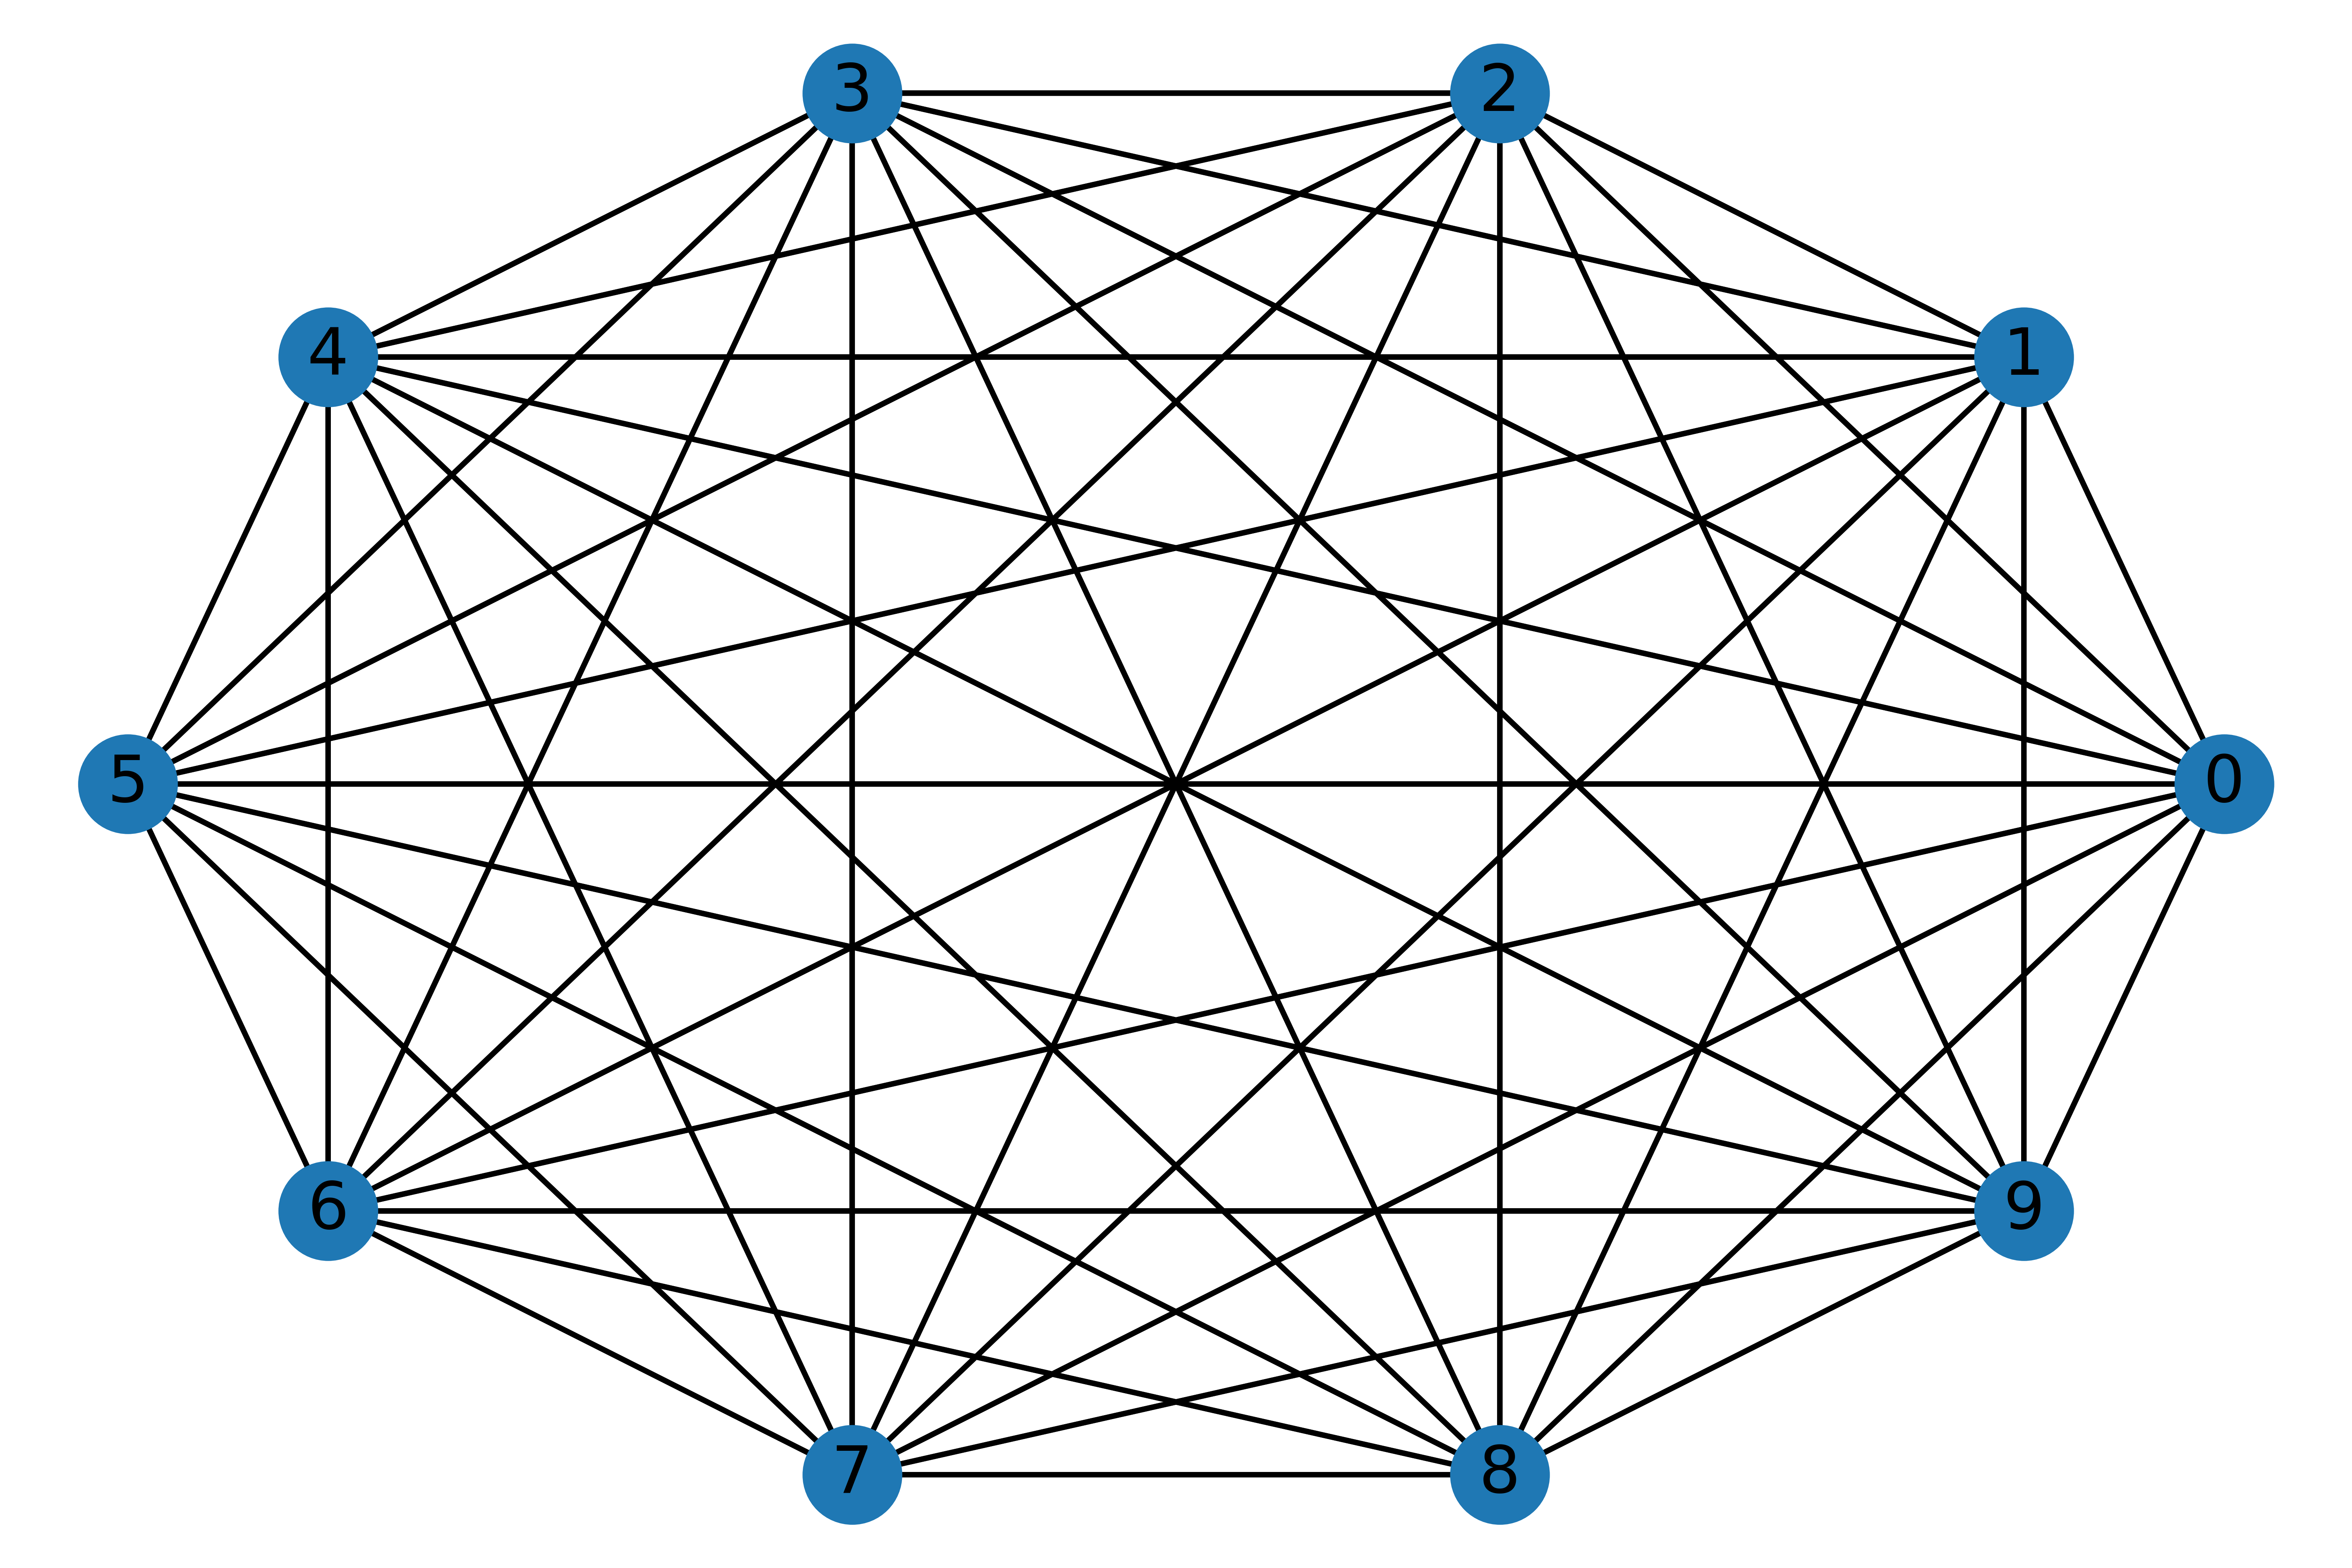
\includegraphics[width=10cm]{primeri/primer2.png}
 	\caption{Poln graf na 5 vozliščih}
	\label{Slika 5}
	\end{figure}
\end{frame}

\begin{frame}
\begin{figure}
  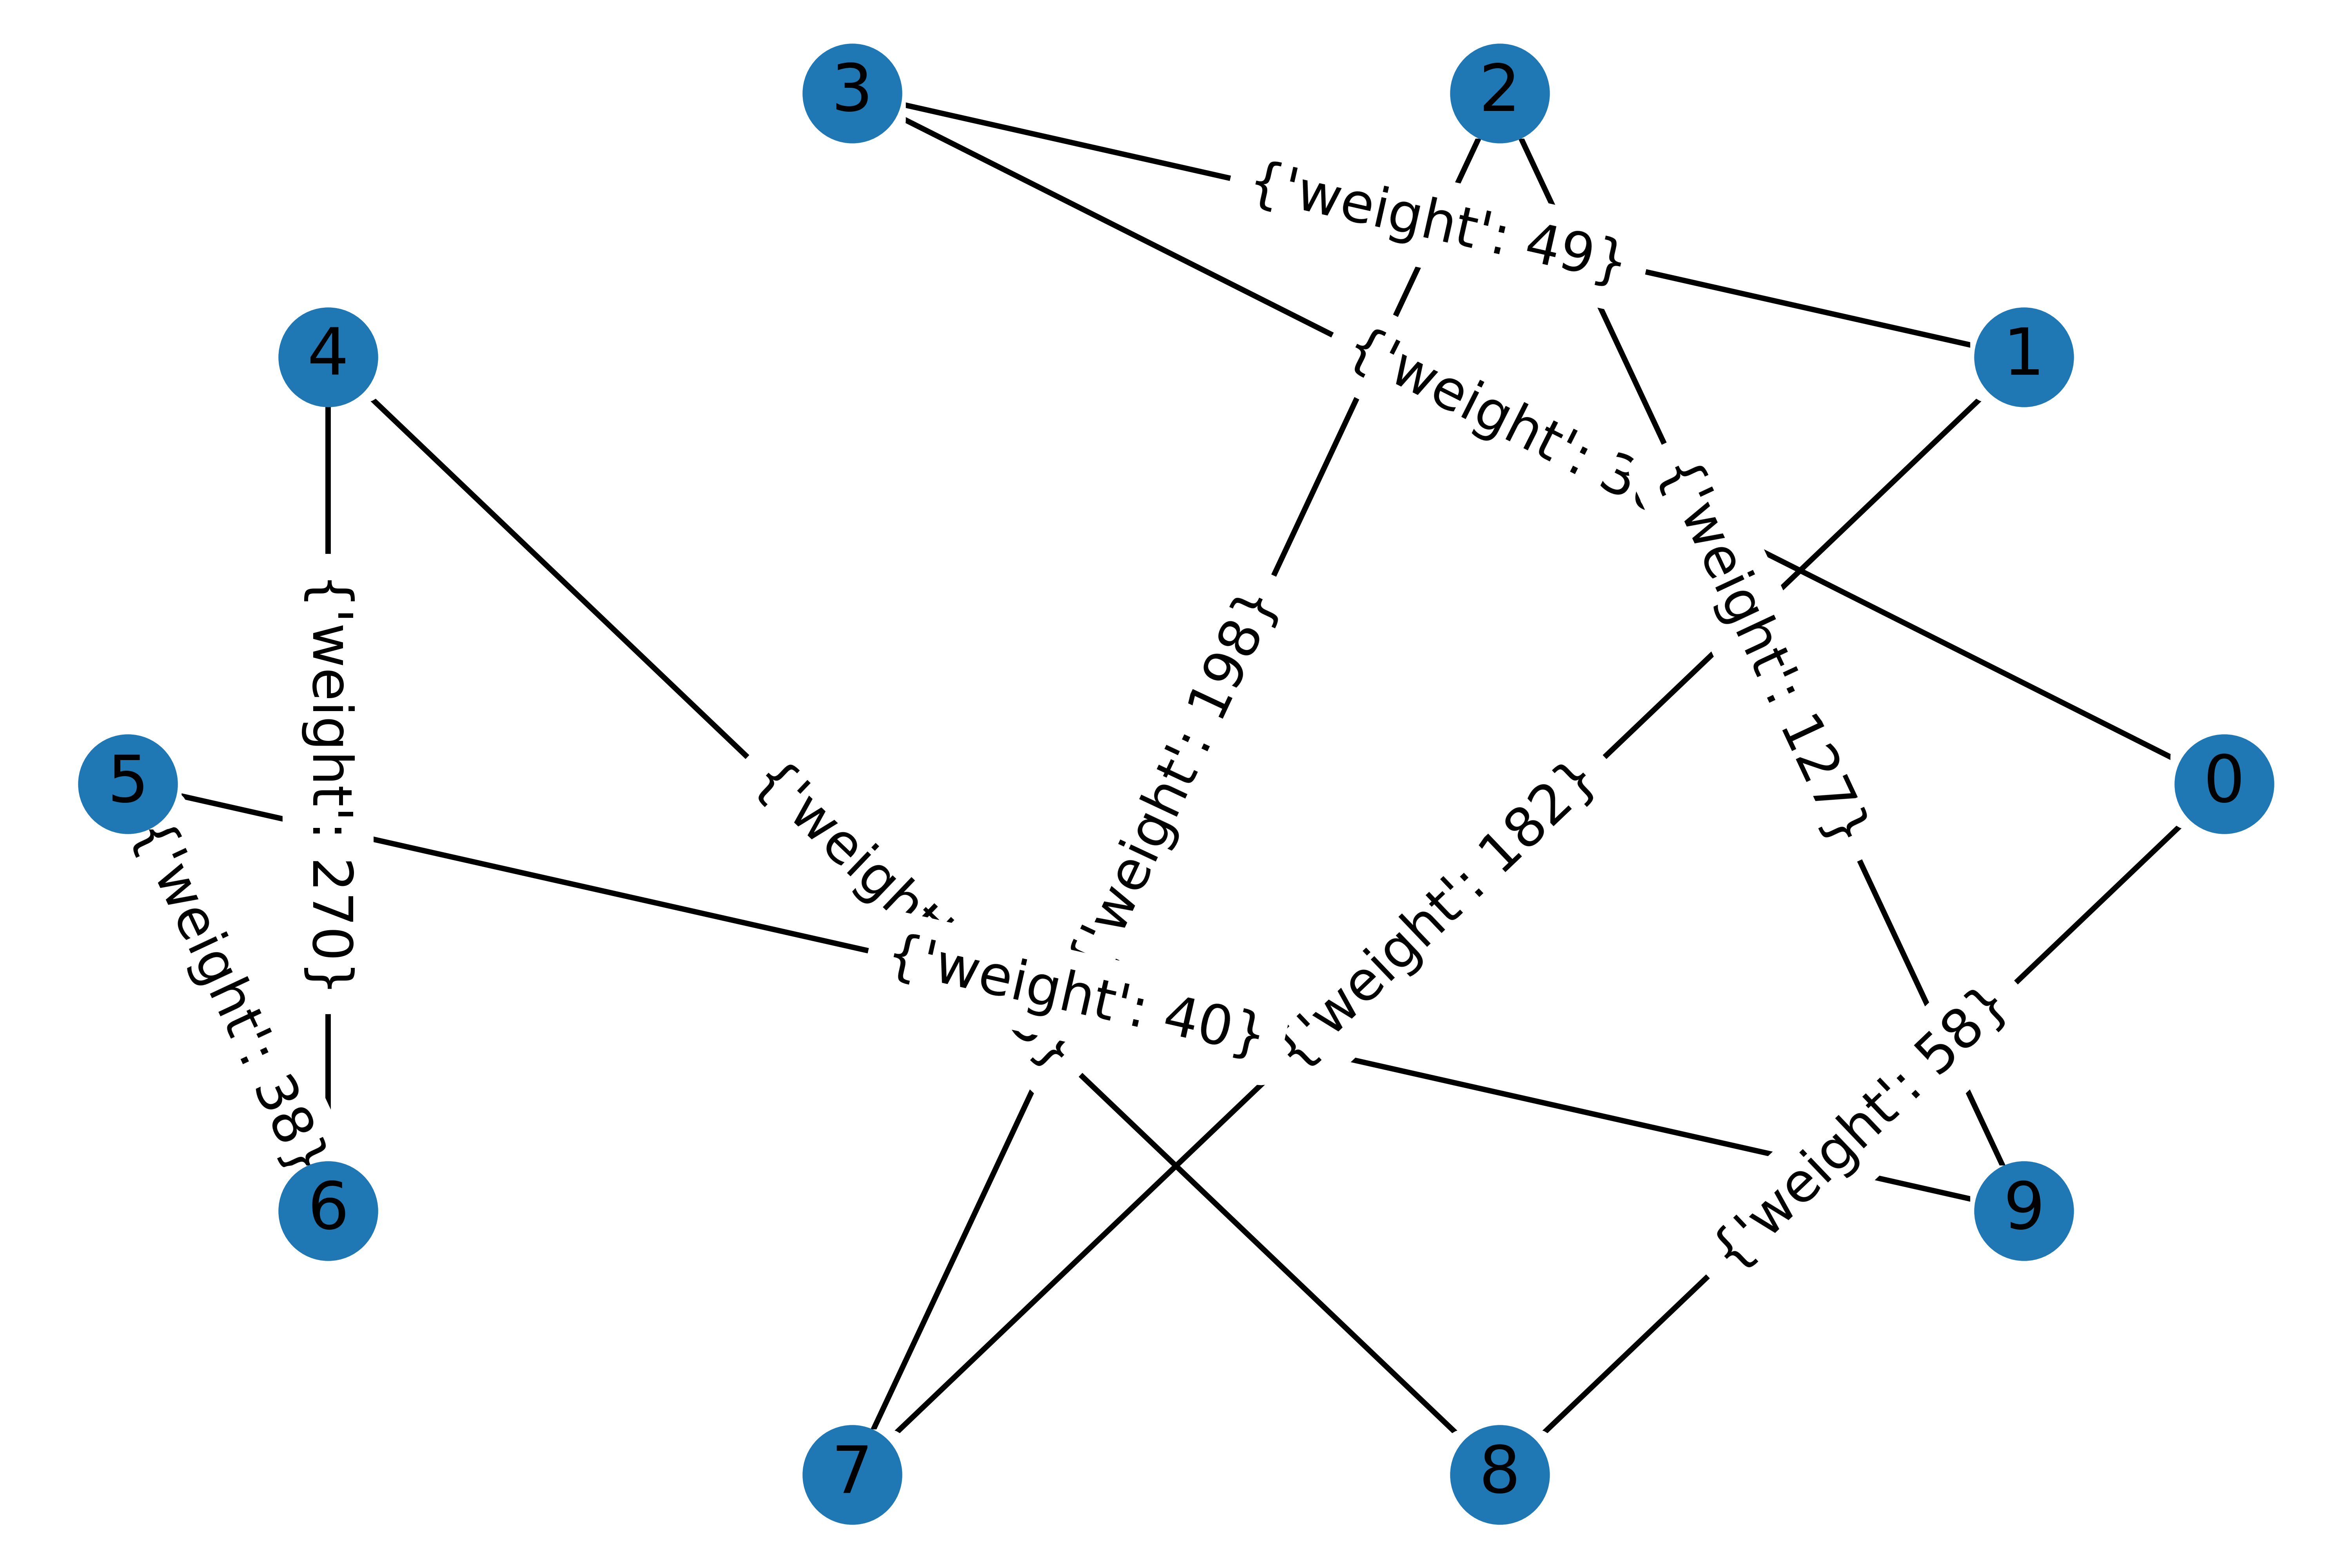
\includegraphics[width=10cm]{primeri/primer2_2opt.png}
\caption{2-opt}
\label{Slika 6}
\end{figure}
\end{frame}


\begin{frame}
  \begin{figure}
  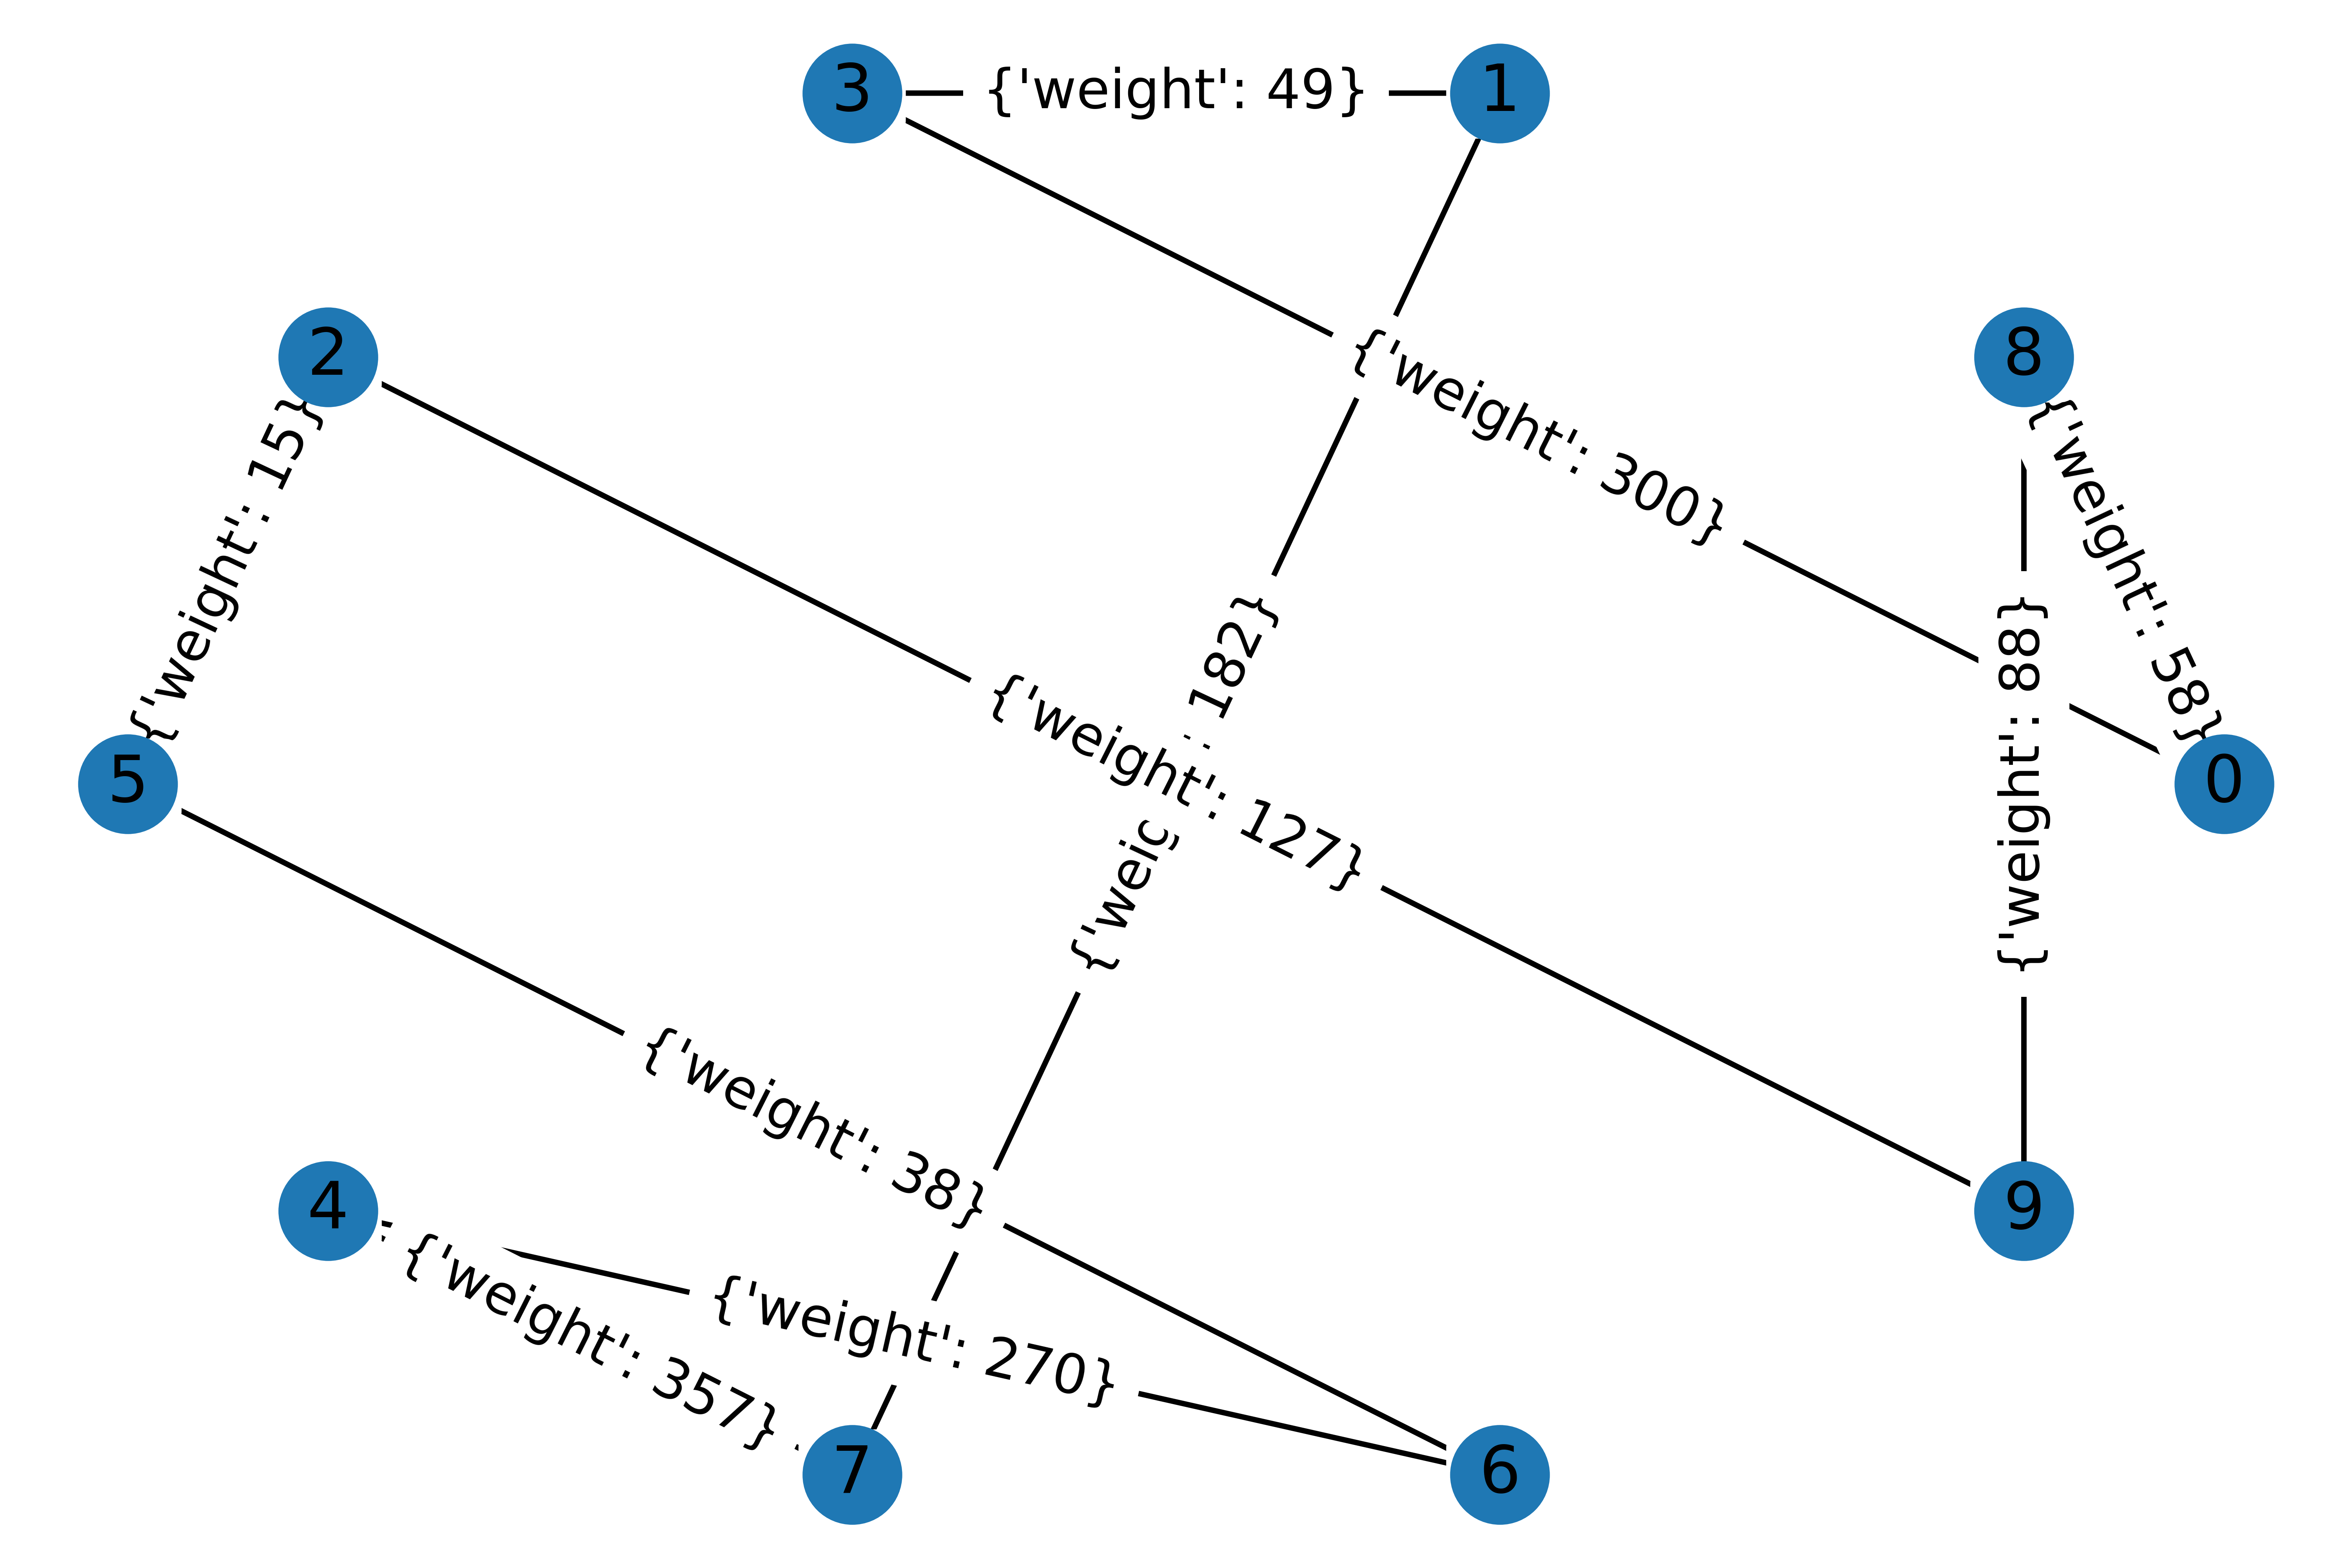
\includegraphics[width=10cm]{primeri/primer2_3opt.png}
 	\caption{3-opt}
	\label{Slika 7}
	\end{figure}
\end{frame}

\begin{frame}
\begin{figure}
  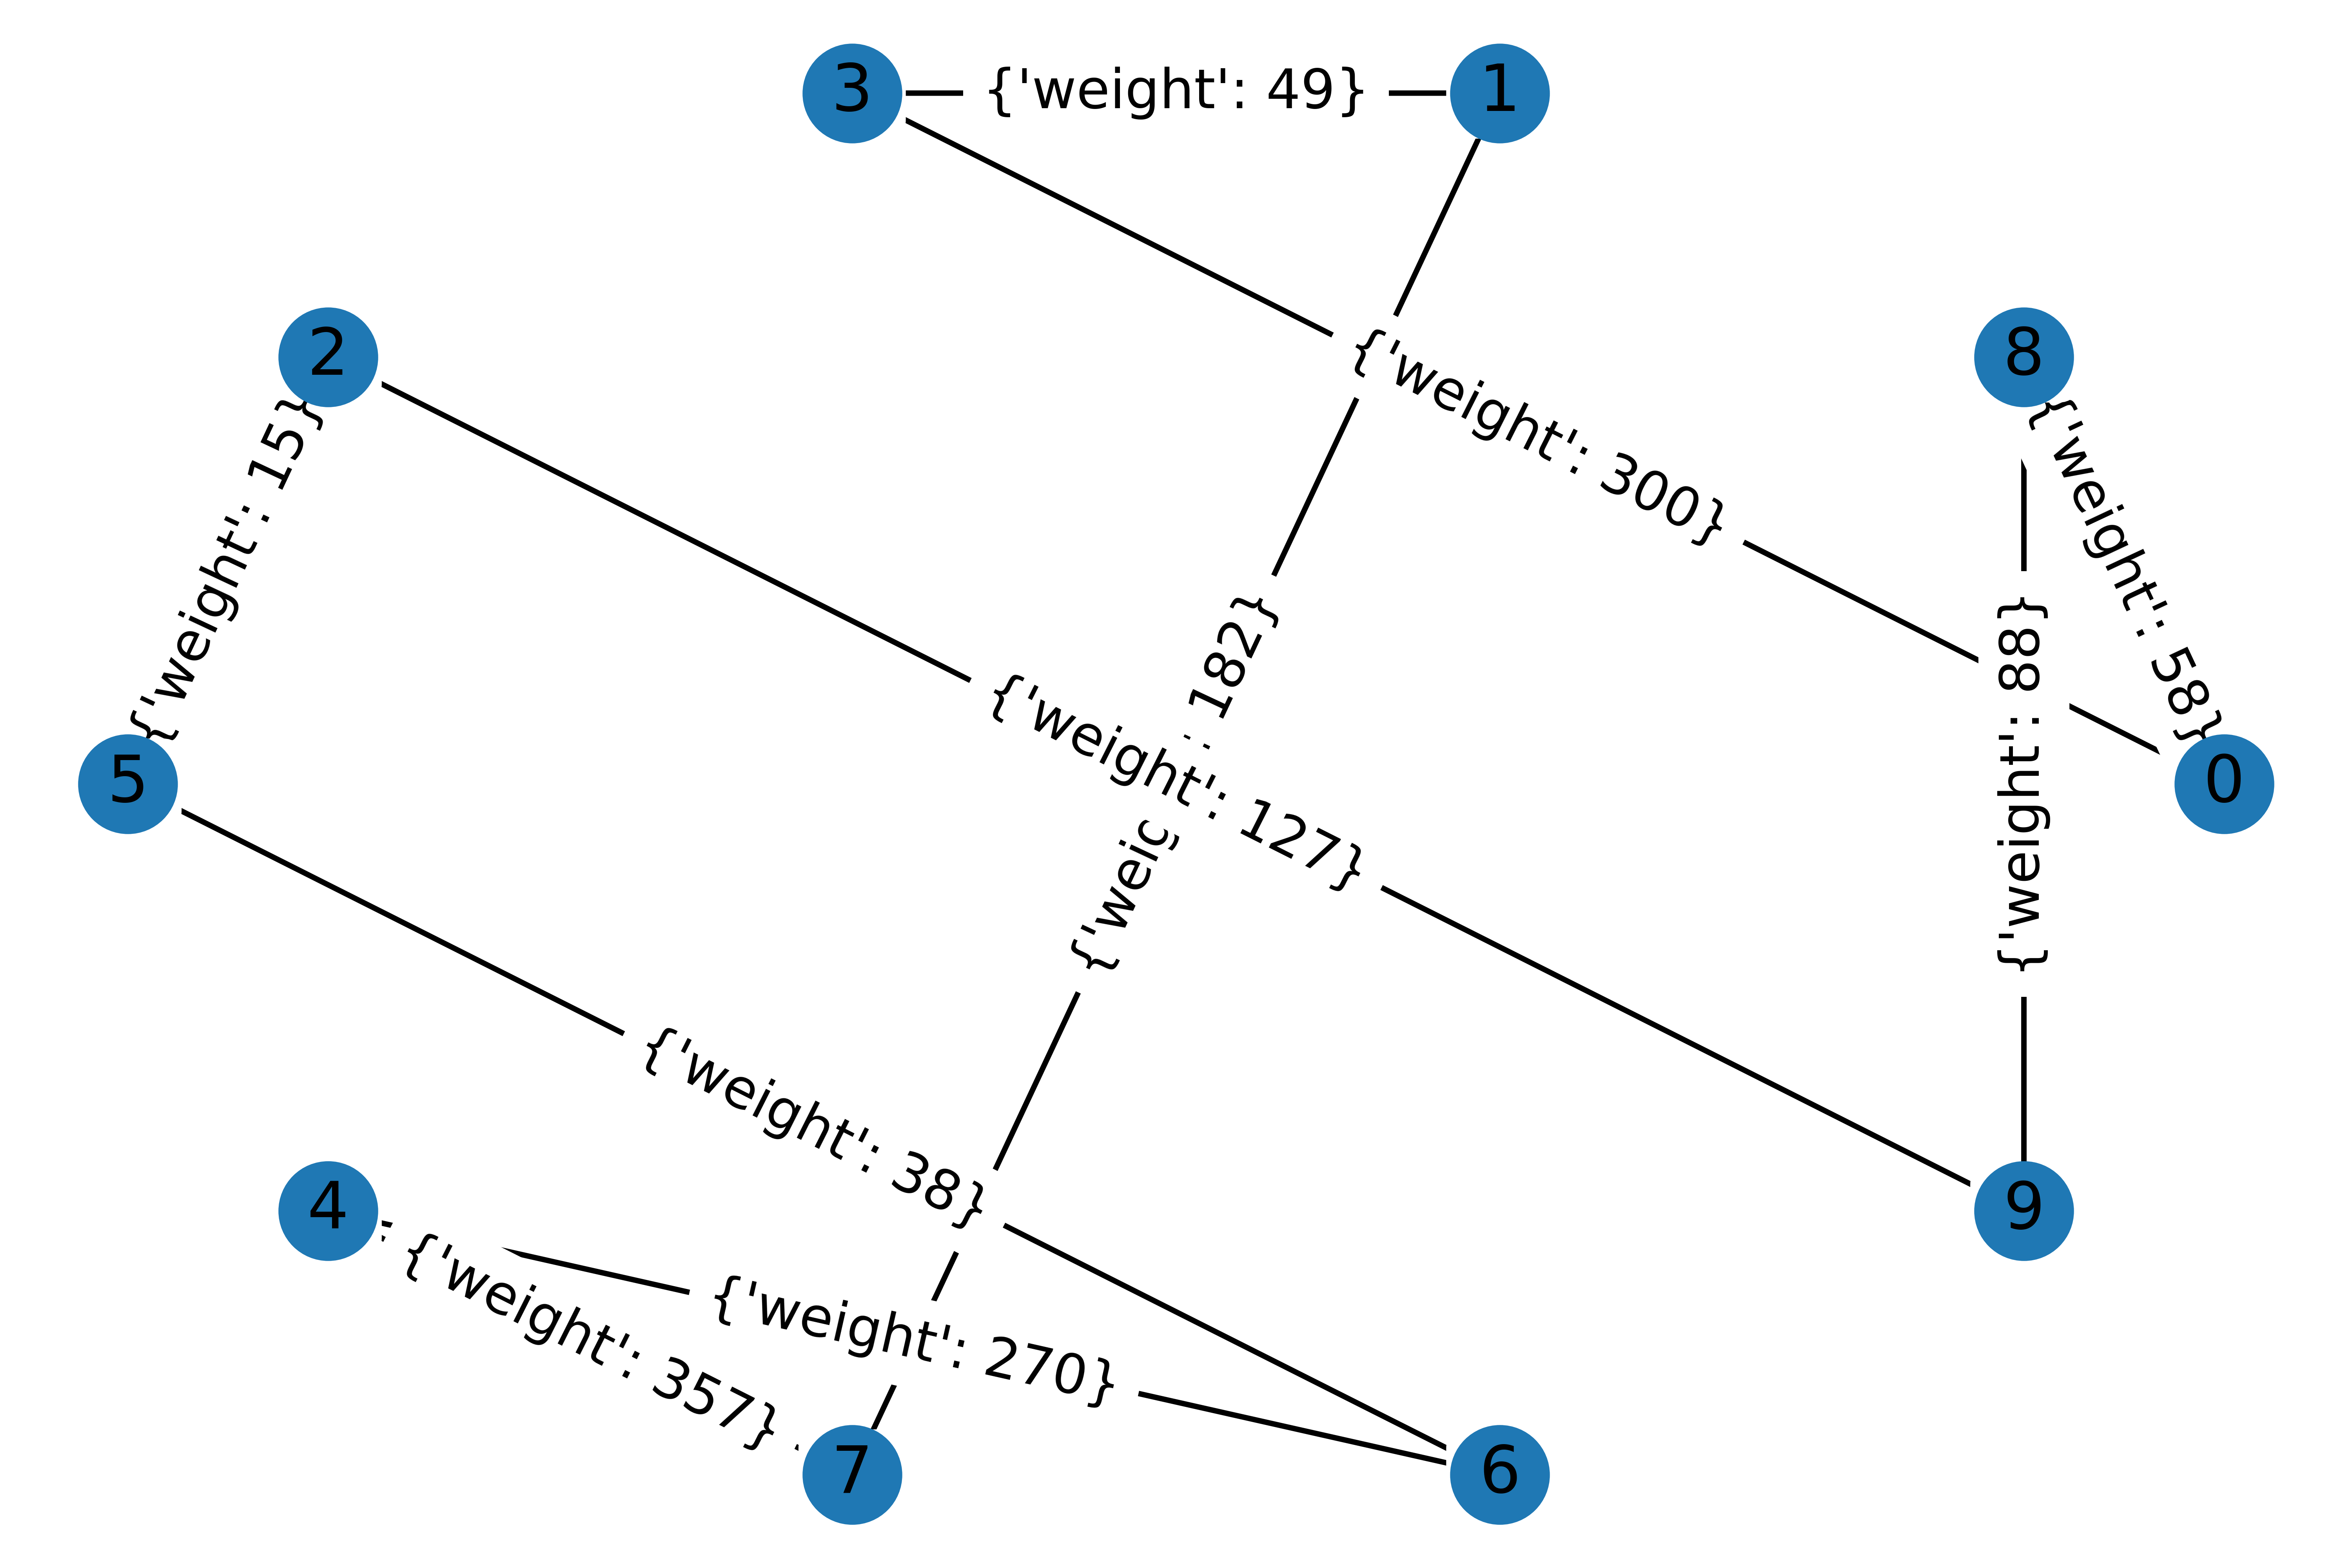
\includegraphics[width=10cm]{primeri/primer2_lk.png}
\caption{LK}
\label{Slika 8}
\end{figure}
\end{frame}

\begin{frame}
\begin{table}[!h]
\begin{tabular}{|c|c|c|c|c|c|c|c|}
\hline
$n$&začetek&2-Opt&cena 2-Opt&3-Opt&cena 3-Opt&LK&cena LK\\\hline
5&49&0,000675&41&0,000276&41&0,000154&41\\\hline
10&4903&0,004748&1595&0,000600&1484&0,000611&1484\\\hline
20&9047&0,03257&1388&0,00801&1555&0,01151&1517\\\hline
30&11825&0,10143&2255&0,01806&1907&0,04639&1729\\\hline
50&23556&0,69378&2833&0,18529&2496&0,30218&2319\\\hline
80&37169&4,97926&3352&0,53484&2890&1,38603&2362\\\hline
100&46984&9,4767&3404&1,97813&2446&2,31723&2235\\\hline
200&98344&194,093&4673&22,9016&3007&13,7700&2832\\\hline
300&156543&1127,92&5365&162,040&2986&94,0348&2630\\\hline
500&244733&7912,40&6689&402,52&3328&496,36&2900\\\hline
\end{tabular}
\caption{Tabela časov izvajanja algoritmov in cen v odvisnosti od $n$}
\label{tabela_casov}
\end{table}
\end{frame}

\begin{frame}
\begin{figure}[!h]
 \begin{center}
  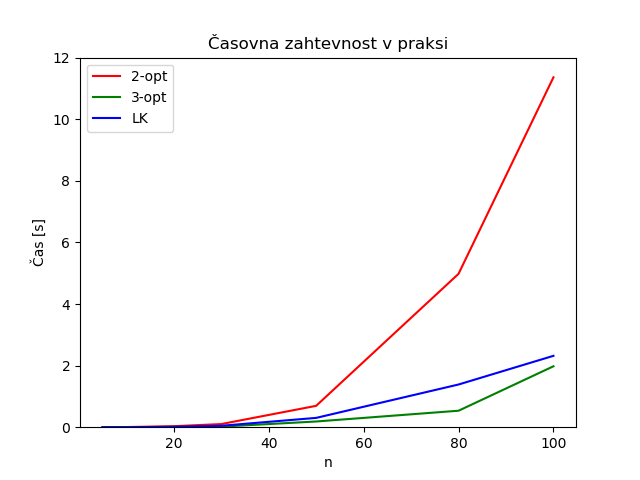
\includegraphics[width=12 cm]{casovna_zahtevnost_do_100.png}
  \caption{Časovna zahtevnost vseh treh algoritmov do $n$ = 100}
  \label{casovna_do_100}
\end{center}
\end{figure}
\end{frame}


\section[Viri]{Viri}
\begin{frame}
\begin{enumerate}

\item A. Hagberg, D. Schult, P. Swart:\emph{NetworkX Refrence, Release 2.4}, [ogled 2.~1.~2020], dostopno na \url{https://networkx.github.io/documentation/stable/_downloads/networkx_reference.pdf}

\item \emph{Optimization with 2-OPT - Part 1}, [ogled 3.~1.~2020], dostopno na \url{http://pedrohfsd.com/2017/08/09/2opt-part1.html}

\item \emph{2-opt}, [ogled 3.~1.~2020], dostopno na \url{https://en.wikipedia.org/wiki/2-opt}

\item \emph{3-opt}, [ogled 4.~1.~2020], dostopno na \url{https://en.wikipedia.org/wiki/3-opt}

\item \emph{3-opt: basic algorithm}, [ogled 4.~1.~2020], dostopno na \url{https://tsp-basics.blogspot.com/2017/03/3-opt-iterative-basic-algorithm.html}

\item D. Karapetyan, G. Gutin, \emph{Lin-Kernighan Heuristic Adaptations for the Generalized Traveling Salesman Problem}, [ogled  8.~1.~2020], dostopno na \url{https://arxiv.org/pdf/1003.5330.pdf}
\end{enumerate}
\end{frame}

\end{document}